% !TeX root = ../../../wyrd.tex

%% Hack for switching page with proper multicols layer
\end{multicols}
\clearpage
\begin{multicols}{2}


\section{Creating Non-Player Characters}\label{core:npcs}\index{Non-Player Characters}\index{NPCs}

\textbf{Non-player characters}, or \textbf{NPCs}, are any characters controlled by the GM that the players interact with. While NPCs can follow the same rules as player characters, this is often unnecessary and can slow down gameplay. Instead, \wyrd\ provides a flexible approach to NPC design, ensuring that simple characters are easy to run while important ones get the attention they deserve.

Not every NPC needs a full stat block. A faceless soldier or a bystander caught in the action doesn’t require the same level of detail as a powerful antagonist or a recurring ally. To keep gameplay fluid and engaging, NPCs in \wyrd\ are divided into three categories:

\begin{enumerate}
    \item \textbf{Mooks:} Nameless threats that exist to provide obstacles or increase tension.
    \item \textbf{Dramatis Personae:} Named characters who have a role in the story but whose details may be fleshed out as needed.
    \item \textbf{Living, Breathing Characters:} Fully realised NPCs with the skills, traits, and motivations to shape the world.
\end{enumerate}


\subsubsection{For NPCs, the rules do not apply}
For all three categories, the key rule of NPCs is this: \textbf{NPCs are not Player Characters}. The rules that apply to player characters see the previous section, do \emph{not} apply to NPCs. NPCs can be both more powerful and far weaker than player characters.

\begin{Example}{NPCs can break the rules}
	\begin{itemize}
		\item NPC skill lists do not need to follow the distribution that player characters' do.
		\item NPCs can have more skills than players and often have fewer.
		\item NPCs can have skill levels below \Untrained and above \Expert.
		\item NPC skills do not have to be taken from the official setting's list of skills---it is often more interesting if NPCs have special skills.
		\item What applies to skills also applies to traits: NPCs can have more powerful traits, have any number of them, and the traits can be more or less powerful than player characters' traits.
		\item The rules for stresses and wounds do not apply to NPCs; NPCs can have any number of stresses and wounds as long as they fit the story.
	\end{itemize}
\end{Example}

NPCs can break the rules in any way that improves the story the game is trying to tell.

Furthermore, \textbf{NPCs do not have to be fully specified} when the game begins. NPCs are usually defined to serve a particular role in the game and will only have the relevant stats for that. A bank clerk the players are supposed to interact with when solving a white-collar crime doesn't need fighting stats. However, if the players somehow get the clerk into a fight, it is perfectly valid to add stats on the fly. This is not cheating; the NPC could have had those stats from the very beginning, but it saves a lot of time for the GM to only worry about the most relevant stats when planning the game.

\begin{GmTips}
	While you \emph{can} improvise stats for NPCs during a game and will have to more often than not, we do not recommend relying on this entirely. Having some idea of what NPCs can do, jotted down as stats, makes it easier to play these characters.	 Game stats can be seen as notes with mechanics effects.
\end{GmTips}


\subsection{Mooks: Quick and Disposable}\index{NPCs!Mooks}
Mooks are the nameless henchmen, foot soldiers, or cannon fodder that serve as obstacles in an encounter. They are not designed to be major threats on their own but can become dangerous in large numbers. The purpose of mooks is to provide \textbf{fast-paced action and cinematic combat} without requiring complex stat tracking.

\subsubsection{Running Mooks in Play}
Mooks are NPCs you do not have to interact with as individuals but rather groups of NPCs players interact with as a collective. Mooks typically:
\begin{itemize}
    \item \textbf{Have a single skill level for all actions.} This is usually set between \Weak and \Skilled.
    \item \textbf{Have minimal or no stress boxes.} A single hit often takes them out.
    \item \textbf{Do not have wounds.} Instead, the GM can describe their defeat narratively.
    \item \textbf{Attack in groups.} Mooks can be treated as a collective, rolling as a single entity for simplicity. The same \Attack or \Defend result is then used for the entire group.
\end{itemize}

\begin{Example}[Example Mook]{Gang Enforcer}
	A hired bruiser working for the city’s criminal underworld, easily replaced if taken down.
	\begin{itemize}
    	\item \textbf{Skill:} \textbf{Combat (+1)} (used for attacks and defence).
	    \item \textbf{Mook Rules:} Drops in one hit if the attack is successful.
	\end{itemize}
\end{Example}

Mooks keep combat \textbf{fast and exciting}, allowing players to feel competent against lesser threats while setting the stage for bigger challenges.

\subsection{Dramatis Personae: Functional but Flexible}\index{NPCs!Dramatis Personae}
\textbf{Dramatis Personae} (or "Characters of the Drama") are named individuals who serve a purpose in the story but don’t need a full character sheet upfront. They might be \textbf{rivals, informants, recurring antagonists, or allies} that the players interact with frequently, but their exact abilities may be determined as needed.

\subsubsection{Key Traits of Dramatis Personae}
Typical Dramatis Personae will have the following traits:
\begin{itemize}
    \item \textbf{Have two or three defined skills} based on their role.
    \item \textbf{May have one or two traits} that give them an advantage in relevant situations.
    \item \textbf{Track stress, but often avoid wounds.} If they take significant damage, they are either removed from play or retreat.
    \item \textbf{Can be adjusted on the fly.} The GM does not need to finalise their full stats until necessary.
\end{itemize}

\begin{Example}[Example Dramatis Personae]{Captain Evelyn Graves}
	A cunning airship captain known for running illegal cargo through dangerous territory.
	\begin{itemize}
    	\item \textbf{Skills:} \textbf{Pilot (+3)}, \textbf{Deception (+2)} , \textbf{Combat (+1)} 
	    \item \textbf{Trait: Born to Fly} – Gains a bonus when piloting under pressure.
        \item \textbf{Trait: Smooth Talker} – Can reroll a failed deception check when negotiating.
    	\item \textbf{Damage:} 2 stress boxes, no tracked wounds.
	\end{itemize}
\end{Example}

The Dramatis Personae NPCs \textbf{fill the world with interesting characters} without overwhelming the GM with excessive bookkeeping.

\subsection{Living, Breathing Characters: Fully Realized NPCs}

Living, Breathing Characters are the \textbf{central figures} of the campaign—the ones who drive the story forward, oppose the players or become long-term allies.

\subsubsection{Key Traits of Living, Breathing Characters}
Living, Breathing Characters are often as fully fledged out as player characters (with the exemptions from strictly following the rules, however):
\begin{itemize}
    \item \textbf{Have full skill allocations} (with the number of skills and levels of skills as appropriate).
    \item \textbf{Have 2-4 defined traits} that impact their playstyle (or as many as needed for the story).
    \item \textbf{Track stress and wounds}, just like player characters (as many and of which kind, as fit the story).
    \item \textbf{May have recurring influence in the game world.}
\end{itemize}

\begin{Example}[Example Living, Breathing Character]{Admiral Lucius Drake}
	The ruthless commander of the Imperial Fleet, obsessed with bringing rogue sky pirates to justice.
  
	\vspace{0.5\baselineskip}
  
	\begin{SkillsBox}
	  \Superior & Strategy \\
	  \Expert & Navigation \\
	  \Skilled & Command, Combat \\
	  \Novice & Resources, Deception, Awareness \\
	\end{SkillsBox}
  
	\begin{TraitsBox}
	  \item[Master Tactician] — Gains a bonus when commanding fleet battles.
	  \item[Iron Will] — Once per session, ignore a mental or social consequence.
	  \item[Unyielding Pursuit] — Can reroll when tracking down a known fugitive.
	\end{TraitsBox}
  
	\begin{GearBox}
	  \item[Imperial Signet Blade] — A ceremonial weapon that grants a \textbf{+2} bonus to \textbf{Command} when used to inspire troops.
	  \item[Sky Admiral’s Compass] — Once per session, automatically succeed on a \textbf{Navigation} check involving uncharted skies.
	\end{GearBox}
  
	\DamageBox
  \end{Example}

Living, Breathing Characters \textbf{serve as the driving force behind conflicts and challenges} in the campaign. They are \textbf{designed to be memorable} and should be treated as full characters in their own right.

\vspace*{\fill}\newcolumn
\subsection{Choosing the Right Type of Non-Player Character}

When introducing an NPC, consider their \textbf{narrative function} first:
\begin{itemize}
    \item If they exist to be fought and defeated quickly, they are mooks.
    \item If they are an ally or minor rival, they are dramatis personae.
    \item If they are a major figure who shapes the world, they are living, breathing characters.
\end{itemize}
\noindent
By keeping NPC design streamlined and flexible, \wyrd\ ensures that GMs can \textbf{focus on storytelling, not stat sheets}. With these guidelines, every character—whether an unnamed mercenary or a legendary villain—can serve their role in the most engaging way possible.

\vspace*{4cm}
\begin{center}
	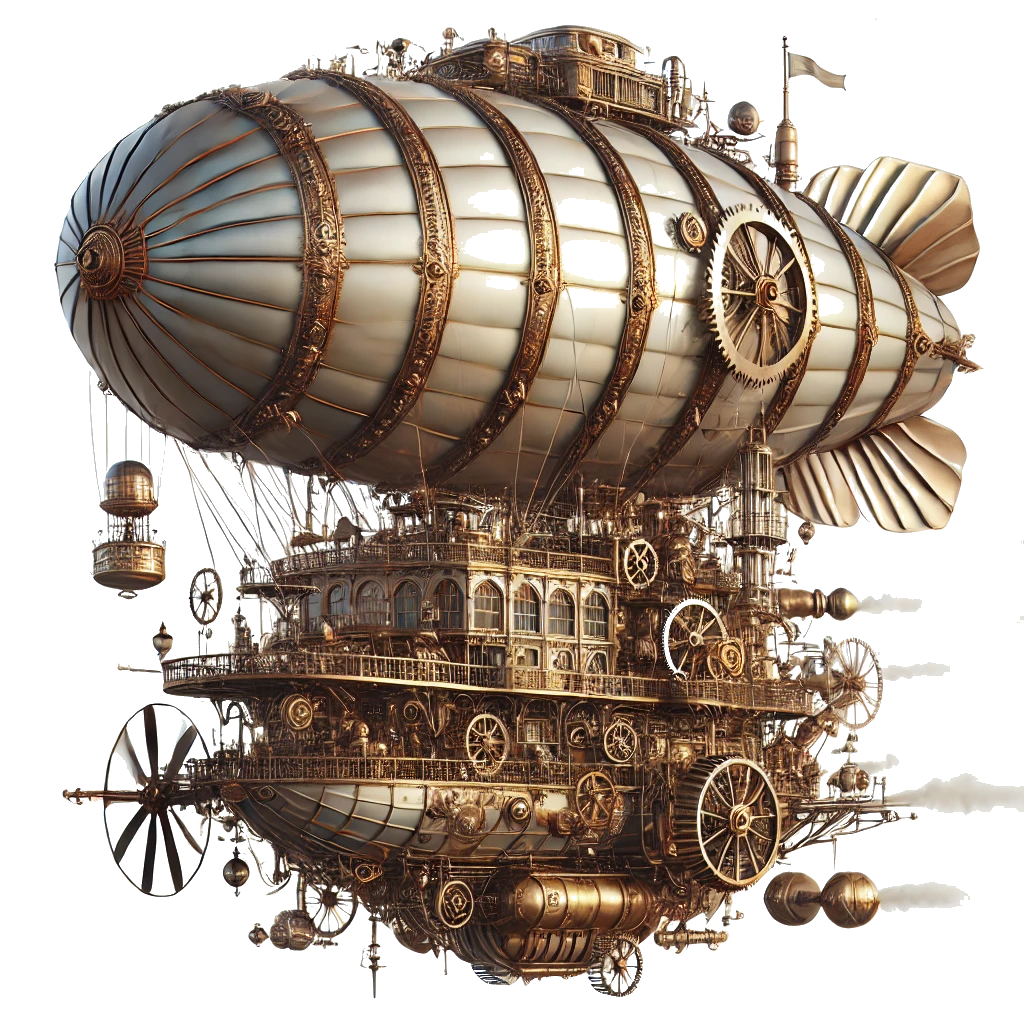
\includegraphics[width=\linewidth]{img/pageart/steampunk_airship_cleaned}
\end{center}
\WyrdFooterImage{img/pageart/steampunk-roofs-mid}